\section{Coined Quantum Walk}

The following example shows how to implement a Coined discrete quantum walk on a cyclic graph with N = 8 nodes. This can be achieved using the coined DQW on a line
where the line is the cyclic graph. First we need to encode the graph nodes in a binary notation to fit with qubits. In general a graph with $2^{n}$ nodes needs n encoding 
bit, in our case since we have $2^{3}$ nodes we can use 3 encoding bit. The Figure 1 below shows how we can bind the qubits to the nodes of the graph.

\begin{figure}[h!]
    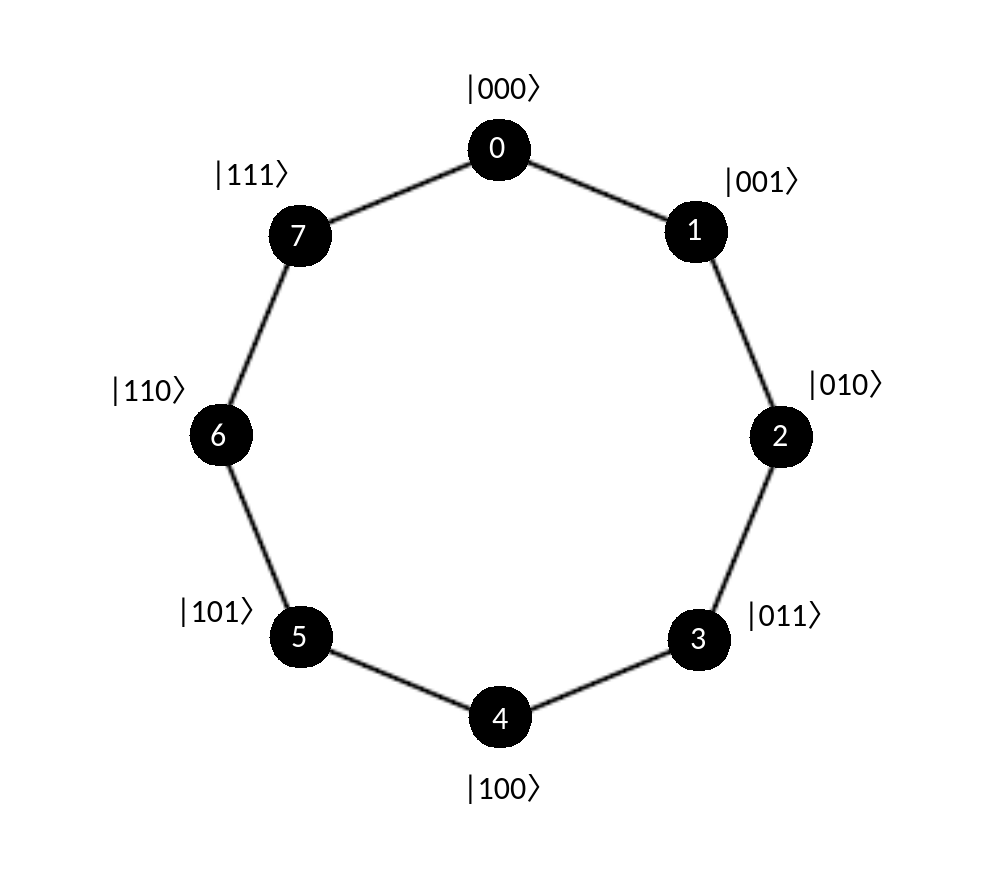
\includegraphics[scale=0.3]{img/cyclic_graph.png}
    \caption{Cyclic graph with 8 nodes, and the respective position state in qubits version}
    \centering
\end{figure}

\subsection{Components description}

We can fit now the 3 main components mentioned in the previous section for this specific example. 

% walker
Starting from the \textbf{walker operator}: for this version we need to encode the nodes of the graph in 3 qubits, the position of the walker 
is given by the binary encoding of the node, for instance the node 0 is represented as $\ket{000}$.

% coin operator
For the \textbf{coin operator}, we will use an Hadamard coin, that
consists in apply the Hadamard operator to the system. 

% hadamard coin description

% shift operator
The \textbf{shift operator} operator in this case will move the actual position that we call $\ket{i}$ to one of the adjacent nodes, that corresponds to 
$\ket{i+1}$ or $\ket{i-1}$, which is decided by the outcome of the coin operator.

\subsection{Circuit for the CQW}

To implement the circuit in qiskit we need to translate the operators defined in quantum circuits, first we need 1 qubit for the coin and 3 for the position, we need log(N) qubits
but for encoding larger number we may need more qubits as support for the multi Toffoli gates, we will see why in the next section.
The Hadamard can be easily implemented using an Hadamard gate on the first qubit. Then we need a circuit to perform an increment and a decrement on the initial state, 
this is less trivial and to achieve that we need two sub circuit that uses multi controlled Toffoli gates. The circuit below represents an incrementer circuit 
for 3 qubits.

\begin{quantikz}
    & \ket{0} & \ctrl{2} & \ctrl{1} & \targ{}  & \qw \\
    & \ket{0} & \ctrl{1} & \targ{}  & \qw      & \qw \\
    & \ket{0} & \targ{}  & \qw      & \qw      & \qw \\
\end{quantikz}

The decrement circuit is similar but uses negative controlled not gates, the circuit below shows the decrement circuit for 3 qubits.

\begin{quantikz}
    & \ket{0} & \octrl{2} & \octrl{1} & \targ{}  & \qw \\
    & \ket{0} & \octrl{1} & \targ{}  & \qw      & \qw \\
    & \ket{0} & \targ{}  & \qw      & \qw      & \qw \\
\end{quantikz}

The negative controlled not can be represented by negate before and after the controlled not, the equivalence circuit below
clarify this explanation, this circuit equivalence came from \cite{nielsen_chuang_2010} which provide other equivalence to build quantum circuits.

$$
\begin{quantikz}[baseline={($(W.base)!.5!(W2.base) -height("$\vcenter{}$")*(0,1pt)$)}]
    & \octrl{1} & \alias{W}  \qw & \qw \\
    & \targ{}   & \alias{W2} \qw & \qw 
\end{quantikz}
=\begin{quantikz}[baseline={($(W.base)!.5!(W2.base) -height("$\vcenter{}$")*(0,1pt)$)}]
    & \gate{X}  & \ctrl{1} & \gate{X} & \qw \\
    & \qw       & \targ{}  & \qw      & \qw 
\end{quantikz}
$$

Finally the decrement circuit defined above, using this equivalence, is showed below.   

\begin{quantikz}
    & \ket{0} & \targ{} & \ctrl{2} & \ctrl{1} & \targ{} & \targ{} & \qw \\
    & \ket{0} & \targ{} & \ctrl{1} & \targ{}  & \qw     & \targ{} & \qw \\
    & \ket{0} & \targ{} & \targ{}  & \qw      & \qw     & \targ{} & \qw \\
\end{quantikz}

To implement the circuit I started with \cite{douglas2007efficient} I didn't know how to build the the negative controlled not before finding that equivalence and \cite{garcia2007high} helped me. 
The circuit above are displayed thanks to the latex package \cite{kay2018tutorial}.
The final circuit is obtained by combining all the components defined and is showed below in Fig.2.

\begin{figure}[h!]
    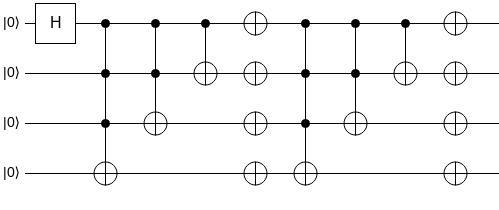
\includegraphics[scale=0.5]{img/cqw.jpg}
    \caption{Complete circuit for the coined quantum walk on a cyclic graph with N=8 nodes}
    \centering
\end{figure}

\href{https://bit.ly/33mno2U}{Click here for a Quirk Simulation}
that shows one step of the circuit above, the sub-circuit are upside down since Quirk uses a little-endian convention.

It's worth to make some comments about it, this circuit represents the U operator, in fact the Hadamard coin will 
randomly choose the direction to take and activate the increment or decrement sub circuit. Therefore this corresponds
to a single iteration of the walk, by successively apply this circuit we can perform a random walk on the cyclic graph.
The code for this circuit can be found in the Appendix A at the end of this document.  

